%%%%%%%%%%%%%%%%%%%%%%%%%%%%%%%%%%%%%%%%%%%%%%%%%%%%%%%%%%
\frame {\frametitle{Background and roadmap}
%%%%%%%%%%%%%%%%%%%%%%%%%%%%%%%%%%%%%%%%%%%%%%%%%%%%%%%%%%
\begin{itemize}
  \item {\bf Reminiscent of traditional database systems}
  \begin{itemize}
  	\item Abstract representation of SQL expressions
  	\item Optimizations for efficiency and performance
  	\item Sophisticated cost model
  \end{itemize}

  \item[]

  \item {\bf Focus on optimizations}
  \begin{itemize}
  	\item Logical plan
  	\item Physical plan
  	\item Cost-based vs. Rule-based
  \end{itemize}
\end{itemize}
}

%%%%%%%%%%%%%%%%%%%%%%%%%%%%%%%%%%%%%%%%%%%%%%%%%%%%%%%%%%
\frame {\frametitle{Global view}
%%%%%%%%%%%%%%%%%%%%%%%%%%%%%%%%%%%%%%%%%%%%%%%%%%%%%%%%%%
\begin{figure}[htbp]
	\centering
	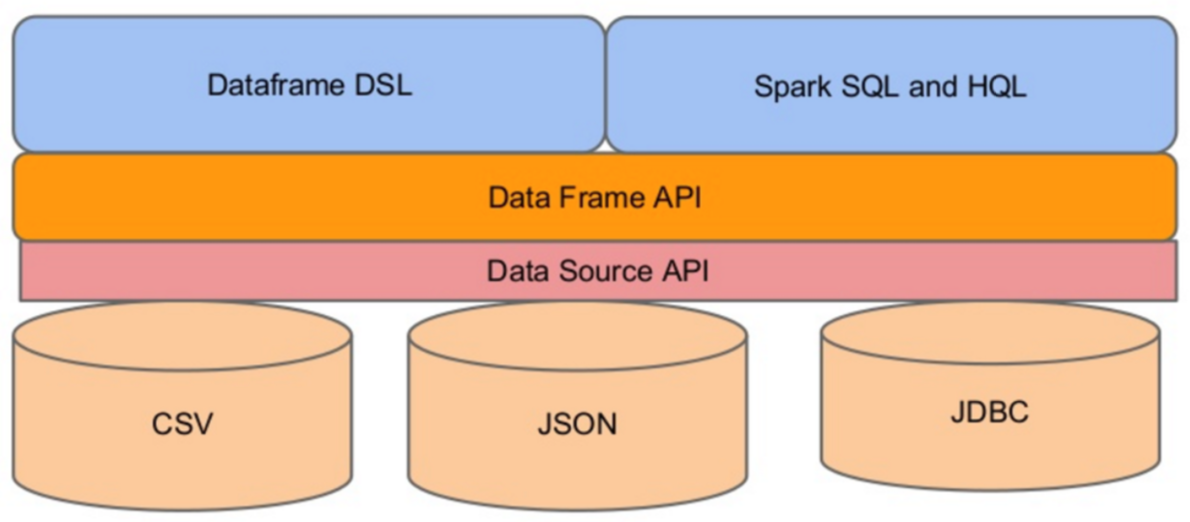
\includegraphics[width=0.95\textwidth]{figures/overview}
\end{figure}
}

%%%%%%%%%%%%%%%%%%%%%%%%%%%%%%%%%%%%%%%%%%%%%%%%%%%%%%%%%%
\frame {\frametitle{SparkSQLContext}
%%%%%%%%%%%%%%%%%%%%%%%%%%%%%%%%%%%%%%%%%%%%%%%%%%%%%%%%%%
\begin{figure}[htbp]
	\centering
	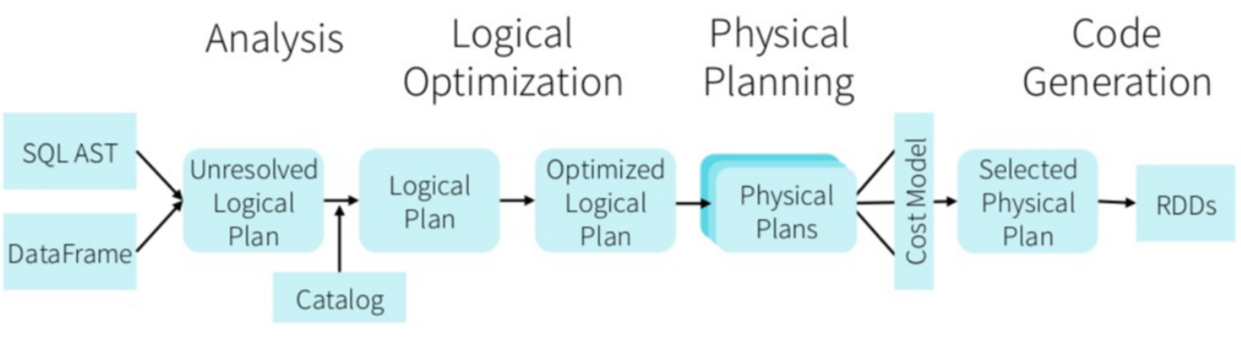
\includegraphics[width=0.95\textwidth]{figures/architecture}
\end{figure}
}

%%%%%%%%%%%%%%%%%%%%%%%%%%%%%%%%%%%%%%%%%%%%%%%%%%%%%%%%%%
\frame {\frametitle{Catalyst optimizer}
%%%%%%%%%%%%%%%%%%%%%%%%%%%%%%%%%%%%%%%%%%%%%%%%%%%%%%%%%%
\begin{itemize}
	\item {\bf Overall goals}
	\begin{itemize}
		\item Optimize logical plan
		\item Convert logical to physical plan
		\item Optimize physical plan
		\item Code generation
	\end{itemize}

	\item[]

	\item {\bf Explot \texttt{scala} language features}
	\begin{itemize}
		\item \texttt{Quasiquotes}
		\item Abstract syntax tree
		\item Tree manipulation library
		\item Optimizations rules implemented as tree transformations
	\end{itemize}
\end{itemize}
}

%%%%%%%%%%%%%%%%%%%%%%%%%%%%%%%%%%%%%%%%%%%%%%%%%%%%%%%%%%
\begin{frame}[fragile=singleslide]{Example query}
%%%%%%%%%%%%%%%%%%%%%%%%%%%%%%%%%%%%%%%%%%%%%%%%%%%%%%%%%%
\begin{columns}

\begin{column}{0.5\textwidth}
\begin{minted}{sql}
SELECT name
FROM (
	SELECT id, name
	FROM People) p
WHERE p.id = 1
\end{minted}
\end{column}

\begin{column}{0.5\textwidth}
   	\begin{center}
     		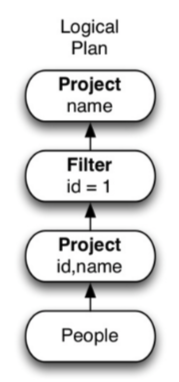
\includegraphics[width=0.5\textwidth]{figures/ex-p1}
   	\end{center}
\end{column}
\end{columns}
\end{frame}

%%%%%%%%%%%%%%%%%%%%%%%%%%%%%%%%%%%%%%%%%%%%%%%%%%%%%%%%%%
\begin{frame}[fragile=singleslide]{Example query}
%%%%%%%%%%%%%%%%%%%%%%%%%%%%%%%%%%%%%%%%%%%%%%%%%%%%%%%%%%
\begin{columns}

\begin{column}{0.5\textwidth}
Native query planning
\begin{minted}{sql}
SELECT name
FROM (
	SELECT id, name
	FROM People) p
WHERE p.id = 1
\end{minted}
\end{column}

\begin{column}{0.5\textwidth}
   	\begin{center}
     		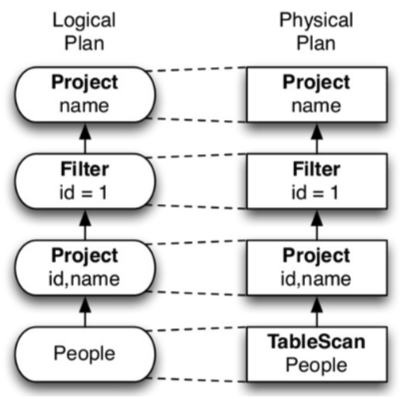
\includegraphics[scale=0.4]{figures/ex-p2}
   	\end{center}
\end{column}
\end{columns}
\end{frame}

%%%%%%%%%%%%%%%%%%%%%%%%%%%%%%%%%%%%%%%%%%%%%%%%%%%%%%%%%%
\begin{frame}[fragile=singleslide]{Example query}
%%%%%%%%%%%%%%%%%%%%%%%%%%%%%%%%%%%%%%%%%%%%%%%%%%%%%%%%%%
\begin{columns}

\begin{column}{0.5\textwidth}
Optimization rules example
\begin{itemize}
	\item Find filters on top of projections
	\item Check that filters can be evaluated without the result of the projection
	\item If yes, switch operators
\end{itemize}
\end{column}

\begin{column}{0.5\textwidth}
   	\begin{center}
     		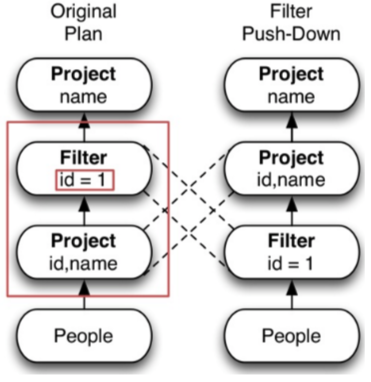
\includegraphics[scale=0.4]{figures/ex-p3}
   	\end{center}
\end{column}
\end{columns}
\end{frame}

%%%%%%%%%%%%%%%%%%%%%%%%%%%%%%%%%%%%%%%%%%%%%%%%%%%%%%%%%%
\begin{frame}[fragile=singleslide]{Example query}
%%%%%%%%%%%%%%%%%%%%%%%%%%%%%%%%%%%%%%%%%%%%%%%%%%%%%%%%%%
\begin{itemize}
	\item Definition of custom rules
\end{itemize}

\begin{figure}[htbp]
	\centering
	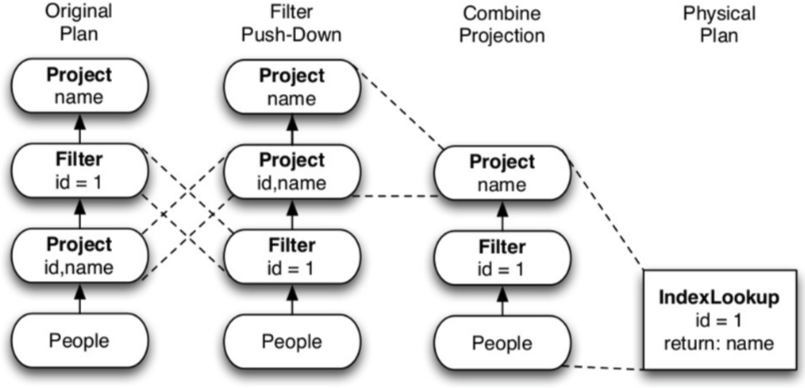
\includegraphics[width=0.95\textwidth]{figures/ex-p4}
\end{figure}

\end{frame}

\frame {\frametitle{Example Optimization Rules}
%%%%%%%%%%%%%%%%%%%%%%%%%%%%%%%%%%%%%%%%%%%%%%%%%%%%%%%%%%
\begin{itemize}
	\item Eliminate subqueries
	\item[]
	\item Constant folding
	\item[]
	\item Simplify filters
	\item[]
	\item PushPredicate through filter
	\item[]
	\item Project collapsing
\end{itemize}
}

%%%%%%%%%%%%%%%%%%%%%%%%%%%%%%%%%%%%%%%%%%%%%%%%%%%%%%%%%%
\frame {\frametitle{Project Tungsten}
%%%%%%%%%%%%%%%%%%%%%%%%%%%%%%%%%%%%%%%%%%%%%%%%%%%%%%%%%%

\begin{itemize}
	\item {\bf Runtime code generation}
	\begin{itemize}
		\item Using code generation to exploit modern compilers and CPUs
	\end{itemize}
	\item[]
	\item {\bf Cache locality}
	\begin{itemize}
		\item Algorithms and data structures to exploit memory hierarchy
	\end{itemize}
	\item[]
	\item {\bf Off-heap memory management}
	\begin{itemize}
		\item Leveraging application semantics to manage memory explicitly and eliminate the overhead of JVM object model and garbage collection
	\end{itemize}
\end{itemize}

}

%%%%%%%%%%%%%%%%%%%%%%%%%%%%%%%%%%%%%%%%%%%%%%%%%%%%%%%%%%
\frame {\frametitle{Advanced features}
%%%%%%%%%%%%%%%%%%%%%%%%%%%%%%%%%%%%%%%%%%%%%%%%%%%%%%%%%%
\begin{itemize}
\item Consider string \texttt{``abcd''}: this is 4 bytes in UTF-8
\end{itemize}

\begin{figure}[htbp]
	\centering
	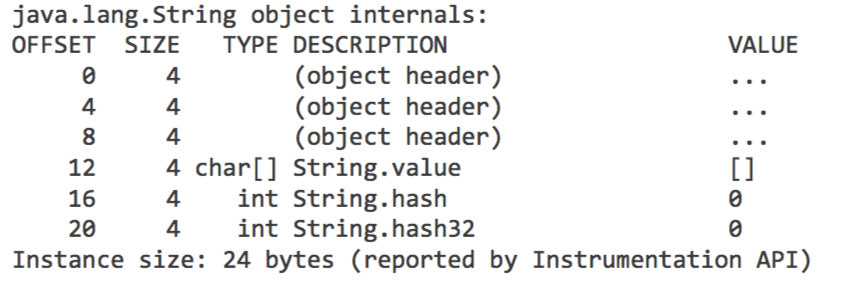
\includegraphics[width=0.95\textwidth]{figures/tungsten}
\end{figure}
}
